\newpage
\subsection{Caso d'uso UC4: Login}
\label{UC4}
\begin{figure}[ht]
	\centering
	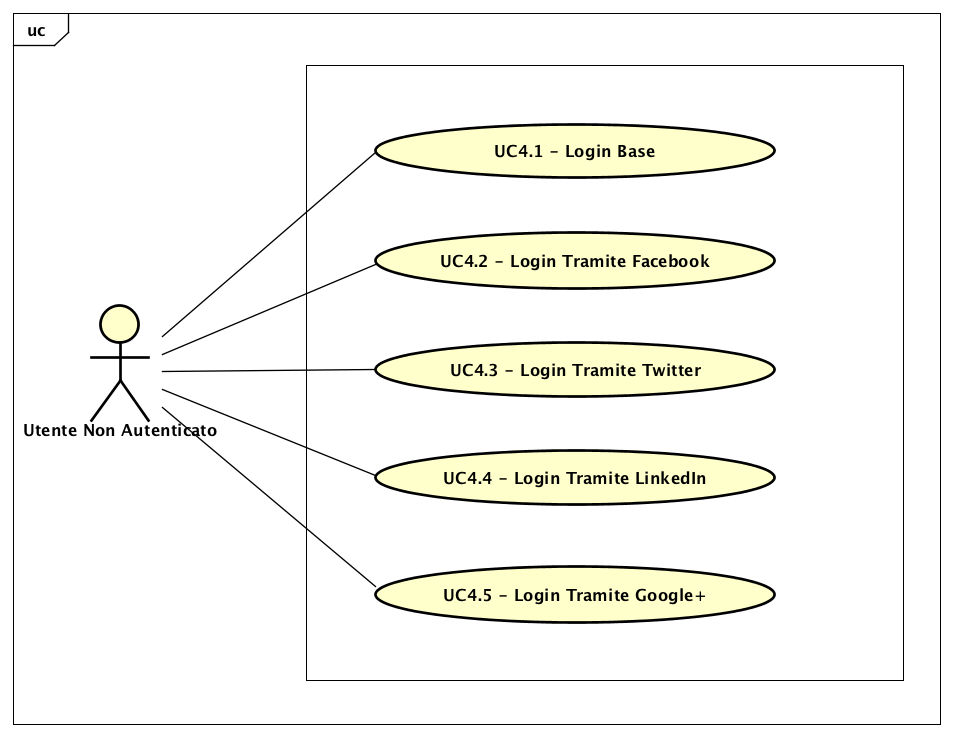
\includegraphics[scale=0.45]{UML/UC4.png}
	\caption{UC4: Login}
\end{figure}

\begin{longtable}{ l | p{11cm}}
	\hline
	\rowcolor{Gray}
	 \multicolumn{2}{c}{UC4 - Login}\\
	 \hline
	\textbf{Attori} & Utente non autenticato \\
	\textbf{Descrizione} & L'attore inserisce le sue informazioni personali per poter accedere all'applicazione web ed evolversi in un utente autenticato \\
	\textbf{Pre-Condizioni} & L'attore si trova nella schermata iniziale dell'applicazione web \\
	\textbf{Post-Condizioni} & L'attore ha effettuato l'accesso all'applicazione web \\
	\textbf{Scenario Principale} & \begin{enumerate*}[label=(\arabic*.),itemjoin={\newline}]
		\item L'attore può effettuare il login tramite API Market (UC4.1)
		\item L'attore può effettuare il login tramite Facebook (UC4.2)
		\item L'attore può effettuare il login tramite Twitter (UC4.3)
		\item L'attore può effettuare il login tramite LinkedIn (UC4.4)
		\item L'attore può effettuare il login tramite Google+ (UC4.5)
	\end{enumerate*}\\
\end{longtable}